\documentclass[../../Thesis.tex]{subfiles}
\usepackage[italian]{babel}

\begin{document}
\chapter{Motivazioni e Lavori Correlati}
In questa sezione della tesi, verranno illustrate in modo approfondito le motivazioni che hanno guidato la scelta del tema di ricerca. Inoltre, saranno presentati e discussi alcuni dei contributi più rilevanti e significativi della letteratura esistente che si sono occupati di effettuare ricerca sul tema.

\section{Motivazioni}
\label{ch:motivations}

Nel 1994, Nick Szabo, un informatico e crittografo, propose la prima descrizione ufficiale degli smart contracts \cite{Szabo_1997}:
 \begin{quotation}
    ``Smart contracts combine protocols, users interfaces, and promises expressed via those interfaces, to formalize and secure relationships over public networks. This gives us new ways to formalize the digital relationships which are far more functional than their inanimate paper-based ancestors. Smart contracts reduce mental and computational transaction costs, imposed by either principals, third parties, or their tools."
 \end{quotation}
L'idea di base dietro uno smart contract è che molte clausole contrattuali possono essere incorporate in hardware e software con cui tutti i giorni interagiamo. Un primo esempio di antenato degli smart contracts possono essere considerati i distributori automatici, che erogano un bene (una bevanda) in cambio di un pagamento. Questo processo è automatizzato e non richiede l'intervento di un intermediario. Il distributore automatico rappresenta un contratto con il portatore: chiunque abbia monete può partecipare a uno scambio con il venditore. La cassetta di sicurezza e altri meccanismi di sicurezza proteggono le monete e il contenuto dagli attacchi, sufficientemente da permettere l'installazione redditizia di distributori automatici in una vasta gamma di aree.

\subsection{Blockchain}
Ad oggi, gli Smart Contracts hanno avuto un'ampissima diffusione grazie allo sviluppo  e alla diffusione della tecnologia blockchain. La blockhain è una tecnologia che permette di costruire un ledger distribuito, cioè un registro condiviso e sincronizzato tra tutti i nodi della rete. Questo registro è immutabile e contiene tutte le transazioni che sono state effettuate. La blockchain è stata introdotta per la prima volta nel 2008 da un autore (o un gruppo di autori) sotto lo pseudonimo di Satoshi Nakamoto, come parte del progetto Bitcoin \cite{Bitcoin}. Le principali carratteristiche della blockchain sono: \cite{Blockchain}:
\begin{itemize}
    \item \textbf{Decentralizzazione}: 
    a differenza dei sistemi di transazione centralizzati, in cui ogni transazione deve essere validata da un'autorità centrale, nella blockchain la validazione delle transazioni avviene in maniera distribuita. In una blockchain, le transazioni sono validate da una rete di nodi distribuiti che collaborano per raggiungere un consenso sulla validità delle transazioni utilizzando specifici algoritmi di consenso.
    \item \textbf{Persistenza:} 
    le transazioni registrate sulla blockchain sono immutabili e non possono essere modificate una volta confermate. I blocchi che contengono transazioni invalide vengono immediatamente rilevati e scartati dalla rete. Questo meccanismo garantisce che il registro sia accurato e affidabile.
    \item \textbf{Anonimità:} ogni utente interagisce con la blockchain con un indirizzo generato, che non rivela la reale indentità dell'utente. Questo garantisce un certo grado di anonimità e privacy. Allo stesso tempo, la blockchain non può garantire un anonimato totale. 
\end{itemize}
A livello architetturale, la blockhain non è altro che una sequenza di blocchi, che tengono una lista completa di record di transazioni, come un ledger pubblico. Ogni blocco contiene un hash crittografico del blocco precedente, un timestamp e un set di transazioni. Questi blocchi sono concatenati insieme per formare una catena, da cui il nome "blockchain". Il primo blocco di una blockchain è chiamato \emph{blocco genesi} ed è l'unico a non avere un blocco precedente. Ogni blocco successivo è collegato al blocco precedente e può avere solo un padre.\\
\begin{figure}[h!]
    \centering
    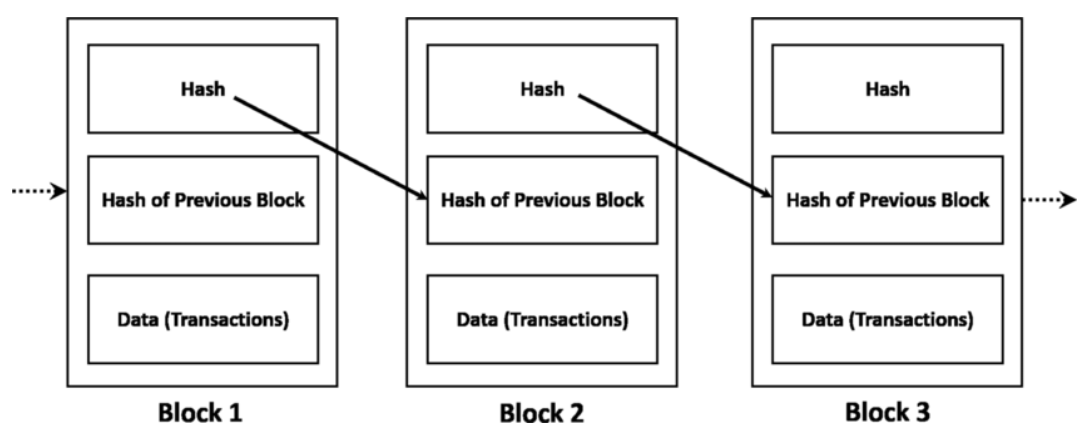
\includegraphics[width=0.8\textwidth]{../../img/Blockchain.png}
    \caption{Esempio di architettura di una blockchain}
    \label{fig:Blockchain}
\end{figure}
Le blockchain possono essere categorizzate in tre tipi principali \cite{Tassonomia}:
\begin{itemize}
    \item \textbf{Blockchain pubbliche}: sono blockchain che chiunque nel mondo può leggere, utilizzare per inviare transazioni e verificare la validità delle transazioni. Tutti i nodi della rete possono partecipare al processo di consenso e alla validazione delle transazioni. Queste blockchain sono considerate completamente decentralizzate. Un esempio di blockchain pubblica è Bitcoin
    \item \textbf{Blockchain private}: e blockchain private sono sistemi in cui i permessi di scrittura sono centralizzati e controllati da un'unica organizzazione. I permessi di lettura possono essere pubblici o limitati a un gruppo selezionato di utenti, a seconda delle esigenze dell'organizzazione. Questo tipo di blockchain viene spesso utilizzato in ambito aziendale per garantire maggiore controllo e sicurezza sulle transazioni e i dati sensibili. Le blockchain private permettono di implementare politiche di accesso più rigorose e di mantenere la privacy delle operazioni interne, rendendole ideali per applicazioni come la gestione della supply chain, la finanza aziendale e la condivisione di dati riservati tra partner commerciali.
    \item \textbf{Blockchain consorziate}: sono blockchain in cui il processo di consenso è controllato da un numero limitato di nodi; ad esempio si può pensare ad un consorzio di istituzioni finanziare in cui ognuna opera come un nodo della rete e per raggiungere un consenso è necessario che la maggioranza dei nodi sia d'accordo. Queste blockchain vengono considerate parzialmente decentralizzate.
\end{itemize}
Una delle sfide principali della blockchain (e, più in generale, dei sistemi distribuiti) è il problema del consenso. Poichè nella blockchain non ci sono dei nodi centrali che garantiscano che i ledger nei nodi distribuiti siano tutti uguali, è necessaria la presenza di un protocollo che assicuri che i ledger siano consistenti tra i vari nodi. Questo protocollo è chiamato protocollo di consenso. Esistono diversi protocolli di consenso, tra i principali possiamo citare:
\begin{itemize}
    \item \textbf{Proof of Work (PoW)}: è il protocollo di consenso utilizzato da Bitcoin. Nel proof of work, i nodi della rete dimostrano di non essere dei malintenzionati spendendo una grande quantità di lavoro computazionale. Questo lavoro è fatto risolvendo un problema crittografico complesso. Nel PoW, ogni nodo della rete calcola l'hash del blocco, che deve però contenere un nonce ed essere inferiore ad un certo valore target. Quando un nodo trova un hash che soddisfa questi requisiti, il blocco viene inviato a tutti gli altri nodi nella rete che devono confermare la validità del blocco. Questo processo è chiamato ``mining" e i nodi che lo fanno sono chiamati ``minatori". Quando un blocco viene confermato, il nodo che ha trovato il blocco riceve una ricompensa in criptovaluta. Tuttavia, PoW richiede una grande quantità di energia elettrica, rendendo il processo costoso e poco sostenibile.

    \item \textbf{Proof of Stake (PoS)}: Il Proof of Stake (PoS) è un protocollo di consenso alternativo a PoW. Poiché PoW richiede un'ampia quantità di lavoro e di energia elettrica, PoS propone un approccio basato sulla quantità di criptovaluta posseduta da un nodo. L'idea di base di PoS è che i nodi che possiedono una grande quantità di criptovaluta sono meno propensi a compiere azioni malevole, poichè ciò potrebbe danneggiare il valore della criptovaluta che possiedono. In PoS, i nodi sono selezionati per validare i blocchi in base alla quantità di criptovaluta che possiedono. Poichè basarsi solo sulla quantità di criptovaluta posseduta potrebbe portare a una centralizzazione del processo di consenso, sono stati proposti diversi algoritmi per selezionare i nodi in modo casuale. Ad esempio, Blackcoin \cite{Blackcoin} utilizza un algoritmo di selezione casuale basato su una lotteria; Peercoin \cite{Peercoin} utilizza un algoritmo di selezione casuale basato sulla quantità di criptovaluta posseduta oltre che sulla quantità di tempo a partire da cui la criptovaluta è stata posseduta. Al contrario di PoW, PoS non richiede una grande quantità di lavoro e di energia elettrica, rendendo il processo di consenso più efficiente e sostenibile, ma al diminuire del costo di mining di un blocco, aumentano le probabilità di attacchi alla blockchain. 
    \item \textbf{Delegated Proof of Stake (DPoS)}: è una variante di PoS in cui i possessori di criptovaluta possono votare per i nodi che desiderano che validino i blocchi. I nodi più votati vengono selezionati per validare i blocchi. Questo riduce il numero di nodi che devono essere coinvolti nel processo di consenso. Questo sistema mira a migliorare l'efficienza e la velocità delle transazioni, mantenendo un certo grado di decentralizzazione. Tuttavia, può introdurre rischi di centralizzazione del potere di voto e governance all'interno della rete.
\end{itemize}
Questi protocolli sono solo alcuni dei tanti protocolli di consenso che sono stati proposti. Ogni protocollo ha i suoi vantaggi e svantaggi e può essere adatto a diversi contesti e applicazioni.

\subsection{Ethereum}


Tra le principali blockchain pubbliche, una delle più importanti è Ethereum. Ethereum è una piattaforma open-source basata su blockchain che permette di creare e distribuire applicazioni decentralizzate (dApp). Proposta per la prima volta nel 2014 da Vitalik Buterin  \cite{Ethereum}, Ethereum estende i concetti introdotti da Bitcoin, pur presentando alcune differenze chiave.

Mentre Bitcoin è progettato principalmente come una valuta digitale, Ethereum è pensata per essere una piattaforma per la creazione di applicazioni decentralizzate. La sua criptovaluta nativa, Ether (ETH), viene utilizzata per pagare le transazioni sulla rete e per incentivare i partecipanti a contribuire alla sicurezza e al funzionamento della rete stessa.

La blockchain di Ethereum è pubblica e permissionless, il che significa che chiunque può partecipare alla rete e inviare transazioni. Inizialmente, la blockchain Ethereum utilizzava il PoW come protocollo di consenso, migrato successivamente al PoS, per migliorare l'efficenza energetica della rete. Ethereum è diventata una delle blockchain più popolari e utilizzate al mondo, con un ecosistema di sviluppatori molto attivo e una vasta gamma di applicazioni decentralizzate che spaziano dai giochi ai servizi finanziari.

\subsection{Smart Contracts}


Una delle principali innovazioni di Ethereum è l'introduzione degli Smart Contracts. Gli smart contracts sono programmi memorizzati ed eseguiti su una blockchain. Possono essere definiti come contenitori di codice che incarnano e replicano i termini di contratti del mondo reale in un dominio digitale \cite{SCReview}. Agiscono come accordi che facilitano lo scambio di denaro, proprietà, azioni o qualsiasi altro valore in modo trasparente, eliminando la necessità di un intermediario. Gli smart contracts vengono eseguiti automaticamente quando vengono soddisfatte determinate condizioni. Ad esempio, un contratto di assicurazione potrebbe pagare automaticamente un risarcimento al verificarsi di un determinato evento. Poiché gli smart contracts sono accessibili ad entrambe le parti, non ci sono dispute una volta che il contratto è stabilito. 

Gli smart contracts di Ethereum possono essere visti come agenti autonomi che vivono sulla blockchain Ethereum. Possono inviare e ricevere transazioni, memorizzare dati e interagire con altri contratti. Gli smart contracts sono scritti in un linguaggio di programmazione chiamato Solidity, progettato appositamente per la creazione di smart contracts. Solidity è un linguaggio di programmazione ad alto livello e Turing-completo, progettato per essere eseguito sulla blockchain Ethereum. Gli smart contracts di Ethereum sono eseguiti su una macchina virtuale chiamata Ethereum Virtual Machine (EVM). L'EVM è una macchina virtuale Turing-completa che esegue il codice Solidity e garantisce che il codice sia eseguito in modo deterministico e sicuro.

Poiché gli smart contracts vengono eseguiti sulla blockchain e sono Turing-completi, sono soggetti al problema dell'arresto (Halting Problem), cioè non è possibile sapere a priori se l'esecuzione di un contratto terminerà o meno. Questo potrebbe rendere le blockchain facilmente soggette ad attacchi di tipo Denial of Service. Per evitare questo problema, Ethereum ha introdotto il concetto di gas. Il gas è una misura dell'uso delle risorse computazionali e di memoria di un contratto. Ogni operazione che un contratto esegue costa una certa quantità di gas. Gli utenti che inviano transazioni devono specificare il prezzo del gas che sono disposti a pagare per l'esecuzione della transazione. Se il gas fornito non è sufficiente per completare l'esecuzione del contratto, la transazione viene annullata e il gas speso non viene restituito all'utente. Al contrario, se l'utente consuma meno del gas disponibile, l'eccedenza viene restituita. Questo meccanismo garantisce che i contratti non possano eseguire operazioni infinite e che gli utenti non possano abusare della rete Ethereum inviando transazioni che richiedono una grande quantità di risorse computazionali.\\
Gli Smart Contracts introducono, numerosi vantaggi \cite{SCReview}:
\begin{itemize}
    \item \textbf{Risparmio}: utilizzando gli smart contracts, si eliminano il tempo e il denaro spesi nell'attesa e nel pagamento di un soggetto terzo per processare una transazione. Le operazioni vengono automatizzate, riducendo così i costi associati ai servizi intermediari e accelerando il processo di transazione.
    \item \textbf{Sicurezza e fiducia:} Una volta che le transazioni sono cifrate e registrate sulla blockchain, sono quasi impossibili da modificare. Questo perché per alterare una singola transazione sarebbe necessario modificare l'intera catena di blocchi, rendendo l'operazione estremamente complessa e dispendiosa per un eventuale attaccante. Inoltre, gli smart contracts, una volta pubblicati, sono immutabili e non possono essere alterati, garantendo che le parti coinvolte possano fidarsi delle condizioni stabilite nel contratto senza timore di manipolazioni future.
    \item \textbf{Accuratezza, efficenza e rapidità:} Dal momento in cui le condizioni stabilite nel contratto sono soddisfatte, l'esecuzione del contratto avviene immediatamente e automaticamente, eliminando la necessità di un intermediario e la compilazione di documentazione cartacea. Questo automatismo non solo accelera i tempi di esecuzione, ma riduce anche il rischio di errori umani associati alla gestione manuale dei documenti.
    
\end{itemize}
\section{Vulnerabilità negli Smart Contracts}

Poichè gli Smart Contracts sono eseguiti su una blockchain pubblica e sono accessibili a tutti, è importante garantire che siano sicuri e privi di vulnerabilità. Come precedentemente già introdotto, una delle caratteristiche principali delli smart contracts è la loro immutabilità. Dopo che un contratto è stato pubblicato sulla blockchain, non può essere modificato o cancellato. Questa proprietà assicura che il comportamento del contratto sia prevedibile e che le parti coinvolte possano fidarsi del contratto. Tuttavia, questa proprietà rende anche gli Smart Contracts vulnerabili a errori e vulnerabilità. Se un contratto contiene una vulnerabilità, essa non può essere corretta e rimarrà vulnerabile per sempre. Questo rende gli Smart Contracts un obiettivo attraente per gli attaccanti che possono sfruttare le vulnerabilità negli Smart Contracts per rubare fondi, bloccare i fondi o causare altri danni \cite{SCEnhancement}.\\
Le vulnerabilità negli Smart Contracts possono essere divise in diverse categorie ed esistono vari criteri di classificazione delle stesse. Una delle classificazioni più comuni è quella proposta da \cite{SmartCheck} che classifica le vulnerabilità in quattro categorie principali:
\begin{itemize}
    \item \textbf{Security}: vulnerabilità che possono portare a perdite di fondi o a comportamenti inaspettati a seguito dell'interazione con un account o un contratto malevolo.
    \item \textbf{Funzionali}: problemi che causano la violazione delle specifiche funzionalità del contratto, per come esse erano state intese.
    \item \textbf{Operazionali}: vulnerabilità che possono portare a problemi operativi, come performance scarse e tempi di esecuzione lunghi.
    \item \textbf{Sviluppo}: problemi legati al codice sorgente del contratto, come codice di bassa qualità che lo rendono difficile da comprendere e migliorare.
\end{itemize}
Queste categorie non tengono in considerazione, però, di informazioni e conoscenze di dominio sugli Smart Contracts. Un'altra classificazione delle vulnerabilità è quella proposta da \cite{sc-vulnerabilities} che propone una classificazione basata su conoscenze di dominio sugli Smart Contracts. Ad esempio, poichè gli smart contracts possono interagire con altri contratti e questa interazione può portare a vulnerabilità come l'attacco di reentrancy o denial of service, queste vulnerabilità sono state classificate come vulnerabilità di tipo \emph{inter-contractual}. Questa classificazione conta cinque categorie principali di vulnerabilità: 
\begin{itemize}
    \item \textbf{Inter-contractual}
    \item \textbf{Contractual}
    \item \textbf{Arithmetic}
    \item \textbf{Gas-Related}
    \item \textbf{Transactional}
\end{itemize}

Paertndo da questa classificazione è possibile identificare diversi tipi di vulnerabilità, più e meno comuni, che possono essere presenti negli Smart Contracts. In questo lavoro di tesi le vulnerabilità sono state classificate in cinque classi diverse:
\begin{itemize}
    \item \textbf{Reentrancy}
    \item \textbf{Unchecked-Calls}
    \item \textbf{Access-Control}
    \item \textbf{Arithmetic}
    \item \textbf{Others}
\end{itemize}

Di seguito, verranno presentate alcune delle vulnerabilità più comuni e significative che possono essere presenti negli Smart Contracts, seguendo la classificazione utilizzata nel resto del lavoro ma con un occhio di riguardo alla classificazione proposta da \cite{sc-vulnerabilities}.

\subsection{Reentrancy}
Le vulnerabilità di tipo reentrancy sono una delle vulnerabilità più comuni e pericolose che possono essere presenti negli Smart Contracts e ricadono nella categoria di vulnerabilità inter-contractual.\\
La Reentrancy è una classe di vulnerabilità presente negli SmartContracts che permette ad un malintenzionato di rientrare nel contratto in modo inaspettato durante l'esecuzione della funzione originale. Questa vulnerabilità può essere utilizzata per rubare fondi e rappresenta la vulnerabilità più impattante dal punto di vista di perdita di fondi a seguito di attacchi.
Il caso più famoso di questo attacco che lo ha anche reso noto è il caso di The DAO \cite{DAO}, un contratto che ha subito un attacco di reentrancy che ha portato alla perdita circa sessanta milioni di dollari in Ether, circa il 14\% di tutti gli Ether in circolazione all'epoca. Nonostante dal 2016 ad oggi siano stati fatti numerosi progressi nelle tecnologie e nelle misure di sicurezza questa vulnerabilità rimane comunque una delle minacce più pericolose per gli SmartContracts, poichè negli anni questo tipo di attacchi si è ripresentato notevole frequenza \cite{reentrancy-historical}. Un attacco di reentrancy può essere classificato in tre classi differenti \cite{Zeus, Vulnerabilities}:
\begin{itemize}
    \item \textbf{Mono-Function}: la funzione vulnerabile è la stessa che viene chiamata più volte dall'attaccante, prima del completamento delle sue invocazioni precedenti. Questo è il caso più semplice di attacco reentrancy e di conseguenza il più facile da individuare.
    \item \textbf{Cross-Function}: questo caso è molto simile al caso di mono-function Reentrancy, ma in questo caso la funzione che viene chiamata dall'attaccante non è la stessa che fa la chiamata esterna. Questo tipo di attacco è possibile solo quando una funzione vulnerabile condivide il suo stato con un'altra funzione, risultando in un una situazione fortemente vantaggiosa per l'attaccante. 
    \item \textbf{Cross-Contract}: questo tipo di attacco prende piede quando lo stato di un contratto è invocato in un altro contratto prima che venga correttamente aggiornato. Avviene solitamente quando più contratti condividono una variabile di stato comune e uno di loro la aggiorna in modo non sicuro. 
\end{itemize}
Mostreremo adesso alcuni esempi di contratti vulnerabili a questo tipo di attacco. Questo esempio mostra un contratto vulnerabile a un attacco di tipo mono-function: 
\begin{lstlisting}[language=Solidity]
// UNSECURE
function withdraw() external {
    uint256 amount = balances[msg.sender];
    (bool success,) = msg.sender.call{value: balances[msg.sender]}("");
    require(success);
    balances[msg.sender] = 0;
}
\end{lstlisting}
In questo caso, il balance dell'utente viene aggiornato solo dopo che la chiamata esterna è stata completata. Questo permette all'attaccante di chiamare la funzione withdraw più volte prima che il balance venga settato a zero, permettendo all'attaccante di rubare fondi allo smart contract.
Una versione più complessa dello stesso processo è il caso cross function, di cui mostriamo un esempio:
\begin{lstlisting}[language=Solidity]
    // UNSECURE
function transfer(address to, uint amount) external {
  if (balances[msg.sender] >= amount) {
    balances[to] += amount;
    balances[msg.sender] -= amount;
  }
}

function withdraw() external {
  uint256 amount = balances[msg.sender];
  (bool success,) = msg.sender.call{value: balances[msg.sender]}("");
  require(success);
  balances[msg.sender] = 0;
}
\end{lstlisting}
In questo esempio, l'attaccante può effettuare un attacco di tipo reentrancy avendo una avendo una funzione che chiama \texttt{transfer()} per trasferire fondi spesi prima che il bilancio sia settato a zero dalla funzione \texttt{withdraw()}.
Gli attacchi Cross-contract sono anche detti Read-only Reentrancy, in cui l'attaccante invece di rientrare nello stesso contratto in cui i cambiamenti di stato sono stati fatti, rientra in un contratto che legge lo stato dal contratto originale. Un esempio di questo caso è il seguente:
\begin{lstlisting}[language=Solidity]
    // UNSECURE
contract A {
	// Has a reentrancy guard to prevent reentrancy
	// but makes state change only after external call to sender
	function withdraw() external nonReentrant {
		uint256 amount = balances[msg.sender];
		(bool success,) = msg.sender.call{value: balances[msg.sender]}("");
		require(success);
		balances[msg.sender] = 0;
	}
}

contract B {
	// Allows sender to claim equivalent B tokens for A tokens they hold
	function claim() external nonReentrant {
		require(!claimed[msg.sender]);
		balances[msg.sender] = A.balances[msg.sender];
		claimed[msg.sender] = true;
	}
}
\end{lstlisting}
Come è possibile vedere, nonostante entrambe le funzioni abbiano il modifier \texttt{nonReentrant}, è cpomunque possibile per un attaccante chiamate \texttt{B.claim} durante la callback in \texttt{A.withdraw} e poichè l'arggiornamento del bilancio dell'attaccante non è stato ancora completato l'esecuzione ha successo.


\subsection{Unchecked-Calls}
Questa classe di vulnerabilità ricade sempre nella categoria di vulnerabilità inter-contractual ed è nota in letteratura anche come \emph{mishandled exceptions, external-calls} ed \emph{exceptions disorders}. 

Questa vulnerabilità si verifica quando un contratto chiama un funzioni di basso livello come \texttt{call, send, delegatecall} senza controllare il risultato di queste chiamate. La differenza tra queste funzioni e la funzione \texttt{transfer} è che quest'ultima propaga un'eccezione nel caso in cui venga generata un'eccezione nel contratto chiamate, al contrario le altre funzioni in caso di fallimento non generano un'eccezione ma ritornano il booleano false \cite{SurveySC}, che se non controllato adeguatamento non stoppa l'esecuzione del contratto \cite{careSC}.  Mostriamo ora un esempio di contratto reso protetto rispetto a questo tipo di vulnerabilità, semplicemente controllando il risultato della chiamata:
\begin{lstlisting} [language=Solidity]
    // Simple transfer of 1 ether
(bool success,) = to.call{value: 1 ether}("");
// Revert if unsuccessful
require(success);
\end{lstlisting}


\subsection{Access-Control}
La vulnerabilità di access-control è una vulnerabilità di tipo contrattuale. Questa vulnerabilità si verifica quando un contratto non controlla correttamente l'accesso alle sue funzioni e ai suoi dati, è quindi una vulnerabilità legata al governare chi può interagire con le varie funzionalità all'interno del contratto. Un esempio di questo tipo di vulnerabilità è legato alla mancata restrizione dell'accesso a funzioni di inizializzazione, ad esempio:
\begin{lstlisting}[language=Solidity]
function initContract() public {
    owner = msg.sender;
}
\end{lstlisting} 
Questa funzione serve a inizializzare l'owner del contratto, ma non controlla chi può chiamarla, permettendo a chiunque di chiamarla e diventare l'owner del contratto, non avendo allo stesso tempo controlli per prevenire la reinizializzazione. Questo è un esempio molto semplice di come una vulnerabilità di access-control possa portare a comportamenti inaspettati. 
Un famoso attacco che ha subito una vulnerabilità di tipo access-control è il caso di Parity Multisig Wallet, un contratto che permetteva di creare wallet multi firma. Questo contratto ha subito un attacco nel Luglio 2017 che ha portato alla perdita di una grande quantità di Ether. L'attacco è stato effettuato da un utente che ha sfruttato una vulnerabilità di access control per diventare l'owner del contratto e rubare criptovalute ad altri utenti, si stima che la perdita sia stata di circa 30 milioni di dollari.

\subsection{Arithmetic}
Le vulnerabilità di tipo aritmetico \cite{sc-vulnerabilities} sono vulnerabilità che vengono generate come risultato di operazioni matematiche. Una delle vulnerabilità più significative all'interno di questa classe è rappresentata dagli \emph{underflow/overflow}, un problema molto comune nei linguaggi di programmazione. Incrementi di valore di una variabile oltre il valore massimo rappresentabile o decrementi al di sotto del valore minimo rappresentabile (detti \emph{wrap around}) possono generare comportamenti indesiderati e risultati errati. In tutte le versioni di Solidity precedenti alla versione 0.8.0, le operazioni aritmetiche non controllano i limiti di overflow e underflow previsti per quel tipo di dato (es.uint64 o uint256), permettendo a un attaccante di sfruttare questa vulnerabilità per ottenere un vantaggio. Ad esempio nel caso in cui si stia utilizzano un uint256 il massimo numero che si piuò memorizzare nella variabile è $2^{256} - 1$, che è un numero molto alto, ma resta comunque possibile superare questo limite, facendo entrare in scena l'overflow. Quando si verifica un overflow, il valore della variabile riparte dal più piccolo valore rappresentabile. Questo può portare a comportamenti inaspettati e a perdite di fondi. Vediamo un esempio molto banale di contratto vulnerabile:
\begin{lstlisting}[language=Solidity]
    pragma solidity 0.7.0;

    contract ChangeBalance {
        uint8 public balance;
        function decrease() public {
            balance--;
        }
        function increase() public {
            balance++;
        }
    }
\end{lstlisting}
Questo codice rappresenta un contratto che molto semplicemente memorizza un saldo all'interno di una variabile di tipo uint8, cioè un intero a 8bit ovvero un intero che può memorizzare valori da 0 a $2^8-1$, quindi da 0 a 255. Se un utente chiamasse la funzione \texttt{increase()} in modo tale che faccia salire il valore del saldo a $256$ il calcolo risulterebbe in un overflow e il valore della variabile ritornerebbe a 0. Questo è un esempio molto semplice di come un overflow possa portare a comportamenti inaspettati. L'underflow si verificherebbe nel caso diametralmente opposto, in cui viene chiamata la funzione \texttt{decrease()} quando il saldo è a 0. In questo caso il valore della variabile ritornerebbe a 255.
Un esempio di attacco che sfrutta l'overflow è stato l'attacco del 23 Aprile 2018 effettuato su uno smart contract di BeautyChain (BEC) che ha causato un importantissimo crash del prezzo, visibile nella figura \ref{fig:BECPrice}. La funzione che ha causato l'overflow permetteva di trasferire una certa somma di denaro presa in input a più utenti contemporaneamnete e per farlo controllava dapprima che il saldo del contratto fosse maggiore o uguale alla somma da trasferire:
\begin{lstlisting}[language=Solidity]
    function batchTransfer(address[] _receivers, uint256 _value) public whenNotPaused returns (bool) {
        uint cnt = _receivers.length;
        uint256 amount = uint256(cnt) * _value;
        require(cnt > 0 && cnt <= 20);
        require(_value > 0 && balances[msg.sender] >= amount);
    
        balances[msg.sender] = balances[msg.sender].sub(amount);
        for (uint i = 0; i < cnt; i++) {
            balances[_receivers[i]] = balances[_receivers[i]].add(_value);
            Transfer(msg.sender, _receivers[i], _value);
        }
        return true;
     }
\end{lstlisting}

\begin{figure}[h]
    \centering
    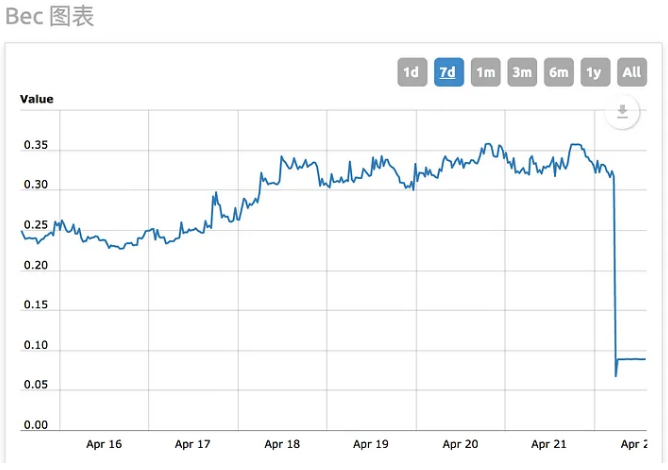
\includegraphics[width=0.8\textwidth]{../../img/BECPrice.png}
    \caption{Andamento del prezzo di BEC prima e dopo  l'attacco}
    \label{fig:BECPrice}
\end{figure}
Dalla versione di Solidity 8.0  tutti i calcoli che superano i limiti di rappresentazione del tipo di dato vengono interrotti e viene lanciata un'eccezione. Questo permette di evitare che si verifichino overflow e underflow. Un'altra soluzione a questo tipo di errori è l'utilizzo della libreria SafeMath, che offre operazioni aritmetiche che controllano i limiti di rappresentazione del tipo di dato prima di effettuare i calcoli. Overflow e underflow sono le principali vulnerabilità di tipo aritmetico, ma non sono le uniche. Un'altra vulnerabilità di tipo aritmetico è rappresentata dalla divisione per zero. In Solidity nelle versioni precedenti alla 0.4 la divisione per zero non lancia un'eccezione, ma ritorna il valore 0, portando a comportamenti inaspettati e a perdite di fondi.
\\
\\
\\
\subsection{Other}
In questa classe di vulnerabilità rientrano tutte quelle vulnerabilità che non fanno parte delle altre classi. Uno degli esempi sono le vulnerabilità di \emph{uninitialized-state}, che si riferiscono a tutte quelle vulnerabilità nate seguito di variabili che non vengono inizializzate correttamente. Le variabili in Solidity possono essere memorizzate in \emph{memory}, \emph{storage} o \emph{calldata}. Bisogna assicurarsi che questi diversi storage vengano compresi e inizializzati correttamente, poichè ad esempio inzializzare male i puntatori allo storage o lasciarli non inizializzati può portare a degli errori. Da Solidity 0.5.0 i puntatori allo storage non inizializzati non sono più un problema poichè contratti con puntatori non inizializzati risulteranno in errori di compilazione.  
\subsubsection*{Incorrect-equality}
Un altra possibile vulnerabilità è detta \emph{incorrect-equality}. Questa vulnerabilità si verifica, solitamente, quando si controlla affinche un account ha abbastanza Ether o Tokens utilizzando una uguaglianza stretta, ciò è un qualcosa che un soggetto malevolo può facilmente manipolare per attaccare il contratto. Un esempio di questo tipo di vulnerabilità è il caso in cui il contratto entra in uno stato di \emph{GridLock}:\\
\\
\begin{lstlisting}[language=Solidity]
    /**
    * @dev        Locks up the value sent to contract in a new Lock
    * @param      term         The length of the lock up
    * @param      edgewareAddr The bytes representation of the target edgeware key
    * @param      isValidator  Indicates if sender wishes to be a validator
    */
   function lock(Term term, bytes calldata edgewareAddr, bool isValidator)
       external
       payable
       didStart
       didNotEnd
   {
       uint256 eth = msg.value;
       address owner = msg.sender;
       uint256 unlockTime = unlockTimeForTerm(term);
       // Create ETH lock contract
       Lock lockAddr = (new Lock).value(eth)(owner, unlockTime);
       // ensure lock contract has all ETH, or fail
       assert(address(lockAddr).balance == msg.value); // BUG
       emit Locked(owner, eth, lockAddr, term, edgewareAddr, isValidator, now);
   }
\end{lstlisting}
In questo caso la vulnerabilità è rappresentata dall'assert che controlla che il contratto abbia ricevuto la quantità di Ether corretta. Il controllo si basa sull'assunzione che il contratto essendo creato alla riga precedente abbia saldo zero ed essendo precaricato proprio con \emph{msg.value} si suppone che il saldo del contratto sia uguale a \emph{msg.value}. In realtà gli Ether possono essere inviati ai contratti prima che vengano istanziati negli indirizzi stessi, poichè la generazione degli indirizzi dei contratti in Ethereum è un processo basato su dei nonce deterministici. L'attacco DoS che si basa su questa vulnerabilità in questo caso consiste nel pre-calcolare l'indirizzo del contatto \emph{Lock} e mandare dei Wei a quell'indirizzo. Questo forza la funzione \emph{lock} a fallire e a non creare il contratto, bloccando il contratto in uno stato di \emph{GridLock}.  Per risolvere questa problematica, si potrebbe adottare l'approccio di sostituire l'uguaglianza stretta con un confronto maggiore o uguale. 

\subsubsection{Denial of Service}
Un'altra classe di vulnerabilità che cade nella categoria di vulnerabilità inter-contractual è la vulnerabilità di tipo Denial of Service (DoS) \cite{sc-vulnerabilities}. Questa vulnerabilità può avvenire per varie ragioni.
Un esempio è il caso in cui si cerca di mandare fondi a un contratto le cui funzionalità dipendono dal successo del trasferimento di questi fondi. Se il trasferimento fallisce, il contratto potrebbe non essere in grado di eseguire le sue funzionalità e rimanere bloccato. Un attaccante potrebbe sfruttare questo comportamento per bloccare il contratto inviando fondi con un contratto che non permette il trasferimento di fondi. Un esempio di questo tipo di vulnerabilità è il seguente:

\begin{lstlisting}[language=Solidity]
    // UNSECURE
    contract Auction {
        address currentLeader;
        uint highestBid;
    
        function bid() payable {
            require(msg.value > highestBid);
    
            require(currentLeader.send(highestBid)); // Refund the old leader, if it fails then revert
    
            currentLeader = msg.sender;
            highestBid = msg.value;
        }
    }
\end{lstlisting}
In questo esempio qualora un'attaccante faccia la bid da uno smart contract con una funzione che annulla tutti i pagamenti, che quindi non può essere rimborsato, il contratto Auction rimarrebbe bloccato e non potrebbe più ricevere offerte. Questo è un esempio molto semplice di come un attaccante possa sfruttare una vulnerabilità di tipo DoS per bloccare un contratto. 

\subsubsection{Suicidal}
Questa vulnerabulità è presente in letteratura anche come \emph{self-destruct}. Precedenti studi \cite{Suicidal} classificano uno smart contract come Suicidal quando utilizza il comando \emph{selfdestruct} senza controllare correttamente il suo utilizzo. 

La vulnerabilità suicida degli smart contract rappresenta un difetto critico che consente la terminazione prematura e irreversibile di un contratto sulla blockchain. Questa vulnerabilità si manifesta quando uno smart contract include una funzione che può essere chiamata da utenti malintenzionati per auto-distruggere il contratto stesso.\\
La funzione \texttt{selfdestruct} in Solidity, ad esempio, è stata progettata per consentire agli sviluppatori di rimuovere contratti obsoleti dalla blockchain e restituire i fondi residui a un indirizzo specificato. Tuttavia, se questa funzione non è adeguatamente protetta o viene esposta accidentalmente, può essere sfruttata per terminare il contratto e compromettere tutte le risorse associate. Per prevenire tale vulnerabilità, è fondamentale implementare rigorosi controlli di accesso e assicurarsi che solo gli utenti autorizzati possano eseguire azioni di questa portata, oltre a condurre audit di sicurezza approfonditi prima del deployment del contratto sulla rete.

Un esempio di smart contract vulnerabile in Solidity è il seguente:

\begin{lstlisting}[language=Solidity]
pragma solidity ^0.8.0;

contract VulnerableContract {
    address payable owner;

    constructor() {
        owner = payable(msg.sender);
    }

    function destroy() public {
        selfdestruct(owner);
    }
}
\end{lstlisting}

In questo esempio, la funzione \texttt{destroy} può essere chiamata da chiunque, causando la distruzione del contratto e il trasferimento dei fondi rimanenti all'indirizzo del proprietario. Per evitare questa vulnerabilità, la funzione \texttt{destroy} dovrebbe essere protetta con un controllo di accesso, come mostrato di seguito:

\begin{lstlisting}[language=Solidity]
function destroy() public {
    require(msg.sender == owner, "Only the owner can destroy the contract");
    selfdestruct(owner);
}
\end{lstlisting}



\section{Lavori Correlati}
\label{ch:relatedwork}
Il tema della rilevazione delle vulnerabilità all'interno degli Smart Contracts è un tema che ha guadagnato notevole importanza nel tempo, anche a seguito della grande diffusione della tecnologia blockchain. Proprio per questo motivo, sono stati sviluppati e proposti diversi approcci per la rilevazione automatica di vulnerabilità all'interno degli Smart Contracts. In questo capitolo verranno presentati alcuni dei lavori più significativi che si sono occupati di questo tema.

Tra i principali approcci proposti figurano gli approcci basati su analisi statica basati su tecniche di esecuzione simbolica. L'analisi statica si basa sull'esame del codice sorgente o bytecode di uno smart contract senza effettuarne l'esecuzione effettiva. Questo approccio consente di identificare potenziali problematiche senza la necessità di testare il codice in un ambiente reale. L'esecuzione simbolica è una tecnica particolarmente potente in questo contesto in quanto consente di esplorare tutte le possibili esecuzioni del programma, consentendo di individuare vulnerabilità che potrebbero emergere solo in determinate condizioni.
Gli approcci basati su esecuzione simbolica cercano di risolvere queste vulnerabilità attraverso la generazione di un grafo di esecuzione simbolico, in cui le variabili sono rappresentate come simboli e le esecuzioni possibili del programma vengono esplorate simbolicamente. Ciò consente di identificare percorsi di esecuzione che potrebbero condurre a condizioni di errore o vulnerabilità.
Tuttavia, va notato che l'analisi statica, inclusa l'esecuzione simbolica, può essere complessa e non sempre completa. Alcune vulnerabilità potrebbero sfuggire a questa analisi o richiedere ulteriori tecniche di verifica. Pertanto, è consigliabile combinare l'analisi statica con altre metodologie, come l'analisi dinamica e i test formali, per garantire una copertura completa nella rilevazione di vulnerabilità negli smart contract. Tra i principali strumenti che utilizzano questo tipo di analisi ci sono Maian \cite{Maian, Maian2}, Oyente \cite{Oyente, Oyente2}, Mythril \cite{Mythril}, Manticore \cite{Manticore} e altri.

Un'altro tipo di approcci ad analisi statica sono i tools basati su regole. Questi strumenti usano un set di regole predefinite e pattern per identificare delle potenziali vulnerabilità nel codice sorgente. Questi tool analizzano il codice sorgente e segnalano tutte le istanze dove il codice viola delle regole predefinite. Le regole sono tipicamente basate su delle vulnerabilità note e delle best practice di programmazione, come ad esempio evitare dei buffer overflow, usare algoritmi di cifratura sicuri e validare propriamente l'input degli utenti. La limitazione principale di questi strumenti è che i risultati che producono sono limitati al set di regole che è stato implementato, quindi non riescono a riconoscere delle nuove vulnerabilità o vulnerabilità non scoperte precedentemente. Inoltre, un'altra grande limitazione di questi strumenti è il fatto che possano produrre un alto numero di falsi positivi, cioè di situazioni in cui il codice viene segnalato come codice vulnerabile ma in realtà è codice perfettamente sano. Tra i principali strumenti che utilizzano questo tipo di analisi ci sono Slither \cite{Slither}, Securify \cite{Securify}, SmartCheck \cite{SmartCheck} e altri.

Un'altra categoria di strumenti per la rilevazione di vulnerabilità negli smart contract sono gli approcci basati su tecniche di Machine Learning e Deep Learning, tra le quali anche il lavoro di questa tesi va ad inserirsi. Un approccio basato sulla trasformazione degli opcode dei contratti e la sua relativa analisi con dei modelli di Machine Learning tradizionale è stato offerto da Wang et al. \cite{ContractWard} i quali hanno raggiunto risultati eccellenti, con risultati in termini di F1 Score superiori al 95\% in quasi tutte le classi prese in analisi con il modello XGBoost che è risultato il miglior modello. Un altro lavoro che sfrutta tecniche di Machine Learning più tradizionali è il lavoro di Mezina e Ometov che hanno utilizzato classificatori come RandomForest, LogisticRegression, KNN, SVM in un approccio dapprima binario (valutare se il contratto abbia o meno delle vulnerabilità) e poi multiclasse (valutare quale tipo di vulnerabilità il contratto abbia) \cite{Mezina}. I risultati in questo caso hanno mostrato come il modello SVM sia quello che ottiene i migliori risultati in termini di accuratezza. 

Spostandoci su lavori che utilizzano tecniche di Deep Learning è importante citare un'altro lavoro effettuato sullo stesso dataset su cui è basato questo lavoro di tesi. Questo dataset è stato infatti raccolto e pubblicato da un gruppo di ricercatori dell'Università di Bologna che ha effettuato un primo studio utilizzando un approccio basato su reti neurali convoluzionali \cite{RossiniPaper1}. L'approccio in questo caso è stato quello di classificare le vulnerabilità in un'impostazione multilabel del problema (in cui la label da predire è un array di elementi, quindi in cui il contratto può appartenere contemporaneamente a più classi) utilizzando delle reti neurali convoluzionali per la rilevazione delle vulnerabilità trasformando in codice Bytecode espresso in esadecimale dei contratti in delle immagini RGB. Questo lavoro ha  come risultato principale la dimostrazione che utilizzando delle reti neurali convoluzionali è possibile rilevare le vulnerabilità presenti negli SmartContracts con delle buone performance, i migliori risultati si attestano con un MicroF1 score del 83\% e mostrano come i migliori risultati siano dati da delle reti Resnet con delle convoluzioni unidimensionali. Successivamente, gli stessi autori hanno pubblicato una seconda analisi effettuata sul dataset utilizzando nuovi classificatori come CodeNet, SvinV2-T e Inception, mostrando come i migliori risultati  continuino ad essere quelli forniti da reti convoluzionali unidimensionali. Altri lavori che utilizzano un approccio basato su tecniche di Deep Learning è il lavoro proposto da Huang \cite{Huang} che utilizza anch'egli delle reti neurali convoluzionali per la rilevazione delle vulnerabilità. I modelli utilizzati sono modelli molto noti come Alexnet, GoogleNet e Inception v3, i risultati migliori in questo caso si attestano sul 75\%.

Un importante lavoro offerto da Deng et Al. \cite{Deng} ha proposto un approccio basato sulla fusione di feature multimodali, analizzando contemporaneamente codice sorgente, bytecode e grafi di controllo del flusso. Per ognuna di queste tre feature è stato addestrato un semplice classificatore con una rete neurale feedforward e sono poi state combinate le predizioni di questi tre classificatori in un classificatore finale utilizzando un approccio di ensamble learning detto stacking. I risultati ottenuti mostrano come l'approccio proposto abbia ottenuto dei risultati migliori rispetto ad un approccio in cui si utilizzava solo una delle tre feature.

Questo lavoro di tesi, non è il primo lavoro che fa uso di modelli di Deep Learning basati su transformers per la classificazione delle vulnerabilità. L'approccio proposto da da Tang et al. \cite{CodeBERTPaper}, ha utilizzato le abilità di encoding del modello CodeBERT per la classificazione del codice sorgente Solidity. Il lavoro ha proposto una classificazione degli encoding di CodeBERT tramite una LSTM, una CNN ed un classico layer totalmente connesso. I risultati hanno mostrato come il layer fully-connected ottenga i migliori risultati con un F1-Score del 93\%. La principale limitazione di questo lavoro è legata al fatto che il dataset utilizzato è molto piccolo, con meno di 10.000 campioni, inoltre, l'altra grande limitazione è che questi modelli non classificavano interi smart contracts, ma solo singole funzioni.

\end{document}